\section{Validity-Guided Synthesis from Assume-Guarantee Contracts}
\label{sec:fixpointsynth}

The lack of soundness for unrealizable results in \jsyn was the catalyst towards pursuing a better approach. The intuition behind the second algorithm in this paper relies on the discovery of a fixpoint $F$ that only contains viable states.  We can determine whether $F$ is a fixpoint by proving the validity of the following formula:
\[
\forall s,i. \ (F(s) \land A(s,i) \Rightarrow \exists s'.G_{T}(s,i,s') \land F(s'))
\]

\noindent In the case where the greatest fixpoint $F$ is non-empty, we check whether it satisfies $G_{I}$ for some initial state.  If so, we proceed by extracting a witnessing initial state and witnessing skolem function $f(s, i)$ to determine $s'$ that is, by construction, guaranteed to satisfy the specification.

To achieve witness extraction, we again depend on \aeval, with its support for generating \textit{regions of validity} being particularly crucial for the computation of fixpoints.

\subsection{Skolem functions and regions of validity}
\label{sec:aeval}


%\andreas{I believe the section can be a bit longer. I also think that the keyphrase ``region of validity'' needs to stand out more. Finally, a proof for Lemma 1, or at least an outline of it would be greatly appreciated.}

We rely on the already established algorithm to decide the validity of $\forall\exists$-formulas and extract Skolem functions, called \aeval~\cite{fedyukovich2015automated}.
It takes as input a formula $\forall x \,.\, \exists y  \,.\, \Phi (x, y)$ where $\Phi (x, y)$ is quantifier-free.
To decide its validity, \aeval first normalizes $\Phi (x, y)$ to the form $S(x) \Rightarrow T(x, y)$ and then attempts to extend all models of $S(x)$ to models of $T(x,y)$.
If such an extension is possible, then the input formula is valid, and a relationship between $x$ and $y$ are gathered in a Skolem function.
Otherwise the formula is invalid, and no Skolem function exists.
We refer the reader to~\cite{KatisFGBGW16} for more details on the Skolem-function generation.

Our approach presented in this paper relies on the fact that during each run, \aeval iteratively creates a set of formulas $\{P_i(x)\}$, such that each $P_i(x)$ has a common model with $S(x)$ and $P_i(x) \Rightarrow \exists y \,.\,T (x,y)$.
After $n$ iterations, \aeval establishes a formula $R_n(x) \eqdef \bigvee_{i=1}^n P_i(x)$ which by construction implies $\exists y\,.\,T(x,y)$.
If additionally $S(x)\Rightarrow R_n(x)$, the input formula is valid, and the algorithm terminates.
%
Fig.~\ref{fg:aeval} shows a Venn diagram for an example of the opposite scenario: $R_2(x) = T_1(x) \lor T_2(x)$, but the input formula is invalid.
However, models of each $S(x) \land P_i(x)$ can still be extended to a model of $T(x, y)$.
%Models of $S(x) \land \neg{R_2(x)}$ cannot be extended to models of $T(x,y)$, thus no formula $T_3(x)$ exists, and \aeval terminates.
% \john {Because we are are already using $A$ and $G$ to represent meaningful formulas I suggest that we use different symbols here so it is not confusing. Especially because the symbols have different signatures in these locations.}

In general, if after $n$ iterations $S(x) \land T(x,y) \land \neg R_n(x)$ is unsatisfiable,
then \aeval terminates.
Note that the formula $\forall x.~ S(x) \land R_n(x) \Rightarrow \exists y .~T(x,y)$ is valid by construction at any iteration of the algorithm.
%Thus, a Skolem function can be generated for it.
%Intuitively, a Skolem function
%describes how $y$ is computed from $s$ in order to satisfy the
%previous formula.
%
We say that $R_n(x)$ is a \emph{region of validity}, and in this work, we are interested in the \emph{maximal} regions of validity, i.e., the ones produced by disjoining all $\{P_i(x)\}$ produced by \aeval before termination and by conjoining it with $S(x)$.
Throughout the paper, we assume that all regions of validity are maximal.
% \john{It is a bit strange how we alternate using formulas that have no free variables along with formulas whose free variables are meant to be implicitly existentially quantified. I think we should either stick with a notation or explicitly say that free variables are interpreted to be existentially quantified.}

% \begin{lemma}
% If formula $\forall x \,.\,  S(x) \Rightarrow \exists y . T(x,y)$ is invalid, and $R_n(x)$ is the region of validity, then there is no other formula $S(x)$ such that $S(x) \land R_n(x) \Rightarrow S(x)$ and $\forall x \,.\,  S(x) \Rightarrow \exists y . T(x,y)$.
% \label{lem:subset}
% \end{lemma}

% \begin{proof}
% Suppose that $S(x)$ exists.
% Then $S(x) \land \neg{R_n(x)} \land S(x)$ is satisfiable, and its models are not contained in $R_n(x)$.
% It contradicts our assumption that \aeval has terminated since otherwise it would proceed for generating $T_{n+1}(x)$ which in turn would enlarge the region of validity.
% \end{proof}

\begin{figure}[!t]
\centering
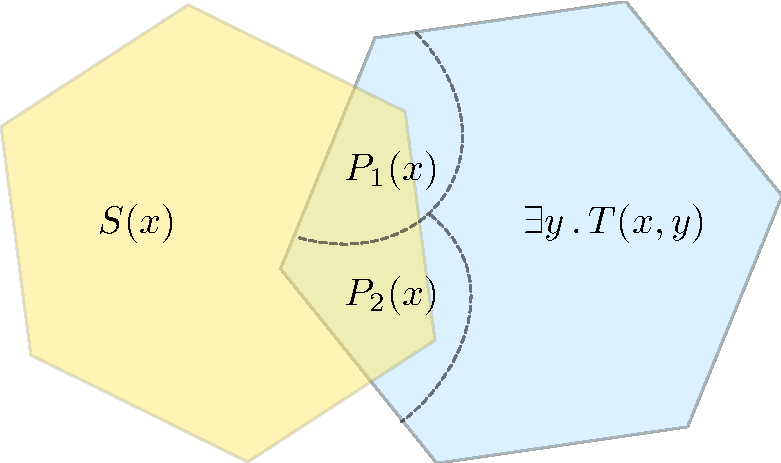
\includegraphics[scale=0.47]{aeval_invalid}
\caption{Region of validity computed for an example requiring \aeval to iterate two times.}
\label{fg:aeval}
\end{figure}

\begin{lemma}\label{lem:aeval}
  Let $R_n(x)$ be the region of validity returned by \aeval for  formula $\forall
  s.~ S(x) \Rightarrow \exists y\,.\,T(x,y)$. Then
%  \begin{equation*}
$  \forall x.~ S(x) \Rightarrow (R_n(x) \Leftrightarrow \exists y\,.\,T(x,y))$.
%  \end{equation*}
\end{lemma}
\begin{proof}
  ($\Rightarrow$) By construction of $R_n(x)$.

  ($\Leftarrow$) Suppose towards contradiction that the formula does
  not hold. Then there exists $x_0$ such that $S(x_0) \land (\exists
  y. T(x_0, y)) \land \neg R_n(x_0)$ holds. But this is a direct
  contradiction for the termination condition for \aeval. Therefore
  the original formula does hold.
\end{proof}

% \begin{corollary}
% If formula $\forall x \,.\,  S(x) \Rightarrow \exists y . T(x,y)$ is invalid, and $R_n(x)$ is the region of validity, then $S(x) \land R_n(x) \Leftrightarrow \exists y . T(x,y)$.
% \label{cor:intermediate}
% \end{corollary}

% \begin{proof}
% ($\Rightarrow$) is immediate from the definition of region of validity.
% ($\Leftarrow$).  Suppose towards contradiction that $s$ satisfies $\exists y . T(x,y)$ but not $S(x) \land R_n(x)$.  If we define $S = s$, we violate Lemma~\ref{lem:subset}.
% \end{proof} 

% \begin{corollary}
% If formula $\forall x \,.\,  S(x) \Rightarrow \exists y . T(x,y)$ is invalid, and $S(x) \land R_n(x)$ is the region of validity, then 
%  $\forall x \,.\, R_n(x) \Leftrightarrow (S(x) \Rightarrow \exists y . T(x,y))$ 
% \label{cor:subset}
% \end{corollary}

% \begin{proof}
% ($\Rightarrow$) Given $s$, suppose $R_n(x)$ is true.  If $S(x)$ is false, then by Corollary~\ref{cor:intermediate},  $\exists y . T(x,y)$ is false, so the implication holds.  Simlarly for $S(x)$ true.
% ($\Leftarrow$) Suppose $S(x) \Rightarrow \exists y . T(x,y)$ is true.  Suppose $S(x)$ is false.  Then $G(s, y)$ might be true and $R_n(x)$ might be false, violating our equivalence.  Boo!
% \end{proof}



\begin{algorithm*}[!t]
\caption{\jsynvg (A : assumptions, G : guarantees)}
\label{alg:synthesis}
\begin{algorithmic}[1]
	\State $F(s) \gets \mathit{true}$\label{alg:init};\Comment{Fixpoint of viable states}
	\While{$\mathit{true}$}
		\State $\phi \gets \forall s,i. \ (F(s) \land A(s,i) \Rightarrow \exists s'.G_{T}(s,i,s') \land F(s'))$\label{alg:ae1};
		\State $\tuple{\mathit{valid}, \subs, \skolems} \gets \aeval(\phi) \label{alg:val1}$;
		\If{$\mathit{valid}$\label{alg:val2}}
            \If{$\exists s . G_{I}(s) \land F(s)$}
				\Return $\tuple{\realizable, \skolems, s, F}$\label{alg:issat};
			\Else{\Comment{Empty set of initial or viable states}}
		 		\Return $\unrealizable$\label{alg:unreal};
		 	\EndIf
		\Else{\Comment{Extract region of validity $Q(s,i)$}}
			\State $Q(s,i) \gets \subs$\label{alg:valreg};
			\State $\phi' \gets \forall s. \ (F(s) \Rightarrow \exists i. A(s,i) \land \lnot
			Q(s,i))$\label{alg:ae2};
			\State $\tuple{\_, \mathit{violatingRegion}, \_} \gets \aeval(\phi')$;
			\State $W(s) \gets \mathit{violatingRegion}$;
			\State $F(s) \gets F(s) \land \lnot W(s)$\label{alg:rem};\Comment{Refine set of viable states}	
		\EndIf
	\EndWhile
\end{algorithmic}
\end{algorithm*}

Alg.~\ref{alg:synthesis}, named \jsynvg (for {\em validity guided}), shows the validity-guided technique that we use towards the automatic synthesis of implementations. The specification is written using the Assume-Guarantee convention that we described in Section~\ref{sec:background} and is provided as an input. For this algorithm we modify the form of the results provided by \aeval to $\tuple{x, y, z} \gets \aeval(\ldots)$: $x$ again specifies if the formula is (not) valid, $y$ identifies the region of validity (in both cases), and $z$ -- the Skolem function (only in case of the validity).

The algorithm maintains a formula $F(s)$ which is initially assigned $\mathit{true}$ (line~\ref{alg:init}).
It then attempts to strengthen $F(s)$ until it only contains viable states (recall Eqs.~\ref{eq:viable}
and~\ref{eq:nonempty}), i.e., a greatest fixpoint is reached.
We first encode Eq.~\ref{eq:viable} in a formula $\phi$ and then provide it as input to \aeval (line~\ref{alg:val1}) which determines its validity (line~\ref{alg:val2}).
If the formula is valid, then a witness $\skolems$ is non-empty.
By construction, it contains valid assignments to the existentially quantified variables of $\phi$.
In the context of viability, this witness is capable of providing viable states that can be used as a safe
reaction, given an input that satisfies the assumptions.

With the valid formula $\phi$ in hand, it remains to check that the fixpoint intersects with the initial states, i.e., to find a model of formula in Eq.~\ref{eq:nonempty} by a simple satisfiability check.
If a model exists, it is directly combined with the extracted witness and used towards an implementation of the system, and the algorithm terminates (line~\ref{alg:issat}).
Otherwise, the contract is unrealizable since either there are no states that satisfy the
initial state guarantees $G_I$, or the set of viable states $F$ is empty.


If $\phi$ is not true for every possible assignment of the universally
quantified variables, \aeval provides a \textit{region of validity} $Q(s,i)$
(line~\ref{alg:valreg}).
%an exact subset of $F(s) \land A(s,i)$, namely $Q(s,i)$, which, if plugged in
% the original left-hand side of $\phi$, makes the resulting formula valid. We will refer to such subsets as \textit{regions of
%validity}.
At this point, one might assume that $Q(s,i)$ is sufficient to restrict $F$ towards a solution. This is not the case since $Q(s,i)$ creates a subregion
involving both state and input variables. As such, it may contain constraints
over the contract's inputs above what are required by $A$, ultimately leading to implementations that only work correctly for a small part of the input domain.

Fortunately, we can again use \aeval's capability of providing regions of validity
towards removing inputs from $Q$.  Essentially, we want to remove those states from $Q$ if even one input causes them to violate the formula on line~\ref{alg:ae1}.  We denote by $W$ the {\em violating region} of $Q$.  To construct $W$, \aeval  determines
the validity of formula $\phi' \gets \forall s. \ (F(s) \Rightarrow \exists
i. A(s,i) \land \lnot Q(s,i))$ (line~\ref{alg:ae2}) and computes
a new region of validity.

If $\phi'$ is invalid, it indicates that there are still non-violating states (i.e., outside $W$) that may lead to a fixpoint.
Thus, the algorithm removes the unsafe states from $F(s)$ in line~\ref{alg:rem}, and iterates until a greatest fixpoint for $F(s)$ is reached.  %If the system is unrealizable, this fixpoint (which may be the formula `false') does not intersect the set of initial states.
If $\phi'$ is valid, then every state in $F(s)$ is unsafe, under a specific input that satisfies the contract assumptions (since $\lnot Q(s,i)$ holds in this case), and the specification is unrealizable (i.e., in the next iteration, the algorithm will reach line~\ref{alg:unreal}).


%or until $W(s)$ becomes valid, that is, for any assignment of the state variables $s$, we have an input that satisfies the assumptions and violates $Q$.  In this case, every state in $F$ has some failing input and the system is unrealizable, which will lead to a failed check in line~\ref{alg:issat} during the next iteration of the loop.


% \subsection{Notes}

% \mike{Here are my notes...sorry that these are disorganized}
% Things to fix:
% \begin{itemize}
% \item The initial state is not returned by the algorithm.
% \item The algorithm checks for validity of $\phi$, but isn't this the same as checking whether the viable region is valid?  Does this boil down to checking whether viableRegion == true?
% \item We need to know where to start a proof.  If it is in terms of the result of Algorithm 1, then it needs to be something returned by Algorithm 1.
% \end{itemize}

% %If the algorithm terminates with a $\realizable$ result, it is straightforward to establish that the generated Skolem function yields a realization.

% Lemmas / proof thoughts.  For soundness of realizable results:
% \begin{itemize}
%     \item It is straightforward to show $Viable$ of the initial state proposed by
%         the algorithm, just by the definition of the fixpoint function, but this doesn't really show the correctness of the Realization (Transition system).
%     \item Showing Realization would be more interesting.
%     \item $\reachable_{A}(s) \Rightarrow F(s)$.  We can prove this with induction.  Base case is easy. Showing inductive case: $\reachable_{A}(s') \Rightarrow F(s')$ from pre-state is also, I think straightforward from:
%         \begin{itemize}
%             \item $\reachable_{A}(s) => F(s)$
%             \item $\reachable_{A}(s)$
%             \item $A(s, i)$
%             \item $T(s, i, s')$
%         \end{itemize}
%         so this immediately implies $F(s')$
%     \item Now we can address the Realization claims, which are all simple non-inductive proofs that follow from definition that T satisfies our fixpoint formula.
% \end{itemize}

% For soundness of unrealizable results:
% \begin{itemize}
%     \item Show Algorithm 1 yields a greatest fixed point
%     \item Show each iteration removes only states that are known to yield a violation.  This is where exactness of AEval is necessary.  This may be a delicate argument; I have not thought it through yet.  I think it would be proved via induction: something like, for each loop iteration, if $\lnot F$ contains only
%         states that violate the guarantees under the assumptions, then $\lnot F'$ contains only states that violate the guarantees under the assumptions.
% \end{itemize}

% Put these two results together and we have that the algorithm yields correct results when it terminates (partial correctness).

% Furthermore, for finite-state problems, the algorithm is totally correct.  For this, we need another proof leg:
% \begin{itemize}
%     \item Each iteration removes at least one state from $F$.  (Progress)
% \end{itemize}

% \mike{End of Mike's notes}

% \subsection{Soundness of Realizable Results}


% \begin{lemma} $\reachable_A(s) \Rightarrow F(s)$
% \end{lemma}

% \begin{theorem} If Alg.~\ref{alg:synthesis} terminates with $\tuple{\realizable, \skolems, I, F}$, then it is a {\em Realization} of the contract $(A, (G_{I}, G_{T}))$.
% \end{theorem}


% \subsection{Soundness of Unrealizable Results}


% \begin{lemma}
% $\viable(s) \Rightarrow s \in F$ is a loop invariant for Alg.~\ref{alg:synthesis} line (2).
% \label{lem:alg1-viable}
% \end{lemma}

% \begin{corollary}
% $s \notin F \Rightarrow \lnot \viable(s)$ is a loop invariant for Alg.~\ref{alg:synthesis} line (2).
% \label{cor:alg1-nonviable}
% \end{corollary}

% \begin{proof}
% Immediate from Lemma~\ref{lem:alg1-viable}.
% \end{proof}

% \begin{theorem} If Alg.~\ref{alg:synthesis} terminates with $\tuple{\unrealizable, ?}$, then there is no $Viable$ state $s$.
% \end{theorem}

% Perhaps we don't even need to bring in Tarski...It could be done with just Hoare logic loop invariants.


\subsection{Soundness}
\label{sec:soundness}

\iffalse
\andrew{TODO: This isn't really a lemma so much as an assumption about
  AE-VAL. We should document it the right way, and then reference it
  as needed in the following proofs.}

\begin{lemma}
$\forall s. \viable(s) \Rightarrow F(s)$ is a loop invariant for Alg.~\ref{alg:synthesis} line (2).
\label{lem:alg1-viable}
\end{lemma}

\begin{proof}
The property is trivially true prior to the first iteration of the loop, because
$F(s) = true$.  Now, suppose $\forall s . \viable(s) \Rightarrow F(s)$ is true at the beginning of the loop.  We have three termination conditions for the loop: the loop exits at lines 8 and 10, and the loop continuation at line~\ref{alg:rem}.  Neither of the termination conditions changes $F$, so these branches are discharged.

What remains is the loop continuation at line~\ref{alg:rem}.  Assuming $\forall s . \viable(s) \Rightarrow F(s)$, we demonstrate $\forall s . \viable(s) \Rightarrow F(s) \land \lnot W(s)$.  We first examine the definition of viability:
\[
    \viable(s) = \forall s,i. \ (A(s, i) \Rightarrow \exists s'.~ G_T(s, i,s') \land \viable(s'))
\]
Applying the assumption yields $(\forall s,i. \ (A(s, i) \Rightarrow \exists s'.~ G_T(s, i,s') \land F(s'))$ (Weakening).

Fixing $s$ to $s_0$, by the induction hypothesis, we know $F(s_0)$.  Suppose $W(s_0)$.  In this case, by line (15) and $F(s_0)$, we know $\exists i. A(s_0, i) \land \lnot Q(s_0, i)$.  We fix $i$ to be some arbitrary constant $i_0$.  From Lemma~\ref{lem:aeval}, we have
$A(s_0, i_0) \land \lnot ((F(s_0) \land A(s_0,i_0)) \Rightarrow \exists s'.G_{T}(s_0,i_0,s') \land F(s'))$.  Since $F(s_0)$ and $A(s_0, i_0)$, simplifying
yields $\lnot (\exists s'.G_{T}(s_0,i_0,s') \land F(s'))$.  But this contradicts the weakened loop hypothesis.  Therefore $\lnot W(s_0)$.  Since $s_0$ was arbitrary, $\forall s . \viable(s) \Rightarrow F(s) \land \lnot W(s)$.
\end{proof}

\begin{corollary}
$s \notin F \Rightarrow \lnot \viable(s)$ is a loop invariant for Alg.~\ref{alg:synthesis} line (2).
\label{cor:alg1-nonviable}
\end{corollary}
\fi


\begin{lemma}
  $\viable \Rightarrow F$ is an invariant for
  Alg.~\ref{alg:synthesis}.
\label{lem:alg1-viable}
\end{lemma}

\begin{proof}
  It suffices to show this invariant holds each time $F$ is assigned.
  On line~\ref{alg:init}, this is trivial. For line~\ref{alg:rem}, we can assume that
  $\viable \Rightarrow F$ holds prior to this line. Suppose towards
  contradiction that the assignment on line~\ref{alg:rem} violates the invariant.
  Then there exists $s_0$ such that $F(s_0)$, $W(s_0)$, and
  $\viable(s_0)$ all hold. Since $W$ is the region of validity for
  $\phi'$ on line~\ref{alg:ae2}, we have
  $W(s_0) \land F(s_0) \Rightarrow \exists i. A(s_0, i) \land \neg Q(s_0, i)$
  by Lemma~\ref{lem:aeval}. Given that $W(s_0)$ and $F(s_0)$ hold, let $i_0$
  be such that $A(s_0, i_0)$ and $\neg Q(s_0, i_0)$ hold. Since $Q$ is the
  region of validity for $\phi$ on line~\ref{alg:ae1}, we have
  $F(s_0) \land A(s_0, i_0) \land \exists s'. G_T(s_0, i_0, s') \land F(s') \Rightarrow Q(s_0, i_0)$
% GF: it used to be this:
% $Q(s_0, i_0) \land F(s_0) \land A(s_0, i_0) \Leftrightarrow \exists s'. G_T(s_0, i_0, s') \land F(s')$
  by Lemma~\ref{lem:aeval}.
  Since $F(s_0)$, $A(s_0, i_0)$ and $\neg Q(s_0, i_0)$ hold, we conclude that
  $\exists s'. G_T(s_0, i_0, s') \land F(s') \Rightarrow \bot$.
  We know that
  $\viable \Rightarrow F$ holds prior to line~\ref{alg:rem}, thus
  $\exists s'. G_T(s_0, i_0, s') \land \viable(s')\Rightarrow \bot$. But this is a
  contradiction since $\viable(s_0)$ holds. Therefore the invariant holds on
  line~\ref{alg:rem}.
\end{proof}


\begin{theorem}
  The \realizable and \unrealizable results of
  Alg.~\ref{alg:synthesis} are sound.
\end{theorem}

% \begin{proof}
% If Alg.~\ref{alg:synthesis} terminates, then the
% formula for $\phi$ on line~\ref{alg:ae1} is valid. Rewritten, $F$
% satisfies the formula
% \begin{equation*}
%   \forall s.~F(s) \Rightarrow \left(\forall i.~ A(s,i) \Rightarrow \exists s'.G_{T}(s,i,s') \land F(s')\right)
% \end{equation*}
% This means $F$ is a post-fixed point of the defining equation for
% $\viable$ given in Equation~\ref{eq:viable}. Moreover $\viable$ is
% defined as the greatest fixed-point of this equation, thus by the
% Knaster-Tarski theorem we have $F(s) \Rightarrow \viable(s)$ for all $s$.
% Combining this with Lemma~\ref{lem:alg1-viable}, we have
% $F(s) = \viable(s)$. Therefore the check on line~\ref{alg:issat} is equivalent to
% the check in Equation~\ref{eq:nonempty} for realizability.
% \end{proof}

\begin{proof}
If Alg.~\ref{alg:synthesis} terminates, then the
formula for $\phi$ on line~\ref{alg:ae1} is valid. Rewritten, $F$
satisfies the formula
\begin{equation}
  \forall s.~F(s) \Rightarrow \left(\forall i.~ A(s,i) \Rightarrow \exists
    s'.G_{T}(s,i,s') \land F(s')\right).
  \label{eq:F-rewritten}
\end{equation}
Let the function $f$ be defined over state predicates as
  \begin{equation}
    f = \lambda V. \lambda s.~ \forall i.~ A(s,i) \Rightarrow \exists s'.G_{T}(s,i,s') \land V(s').
    \label{eq:f-fixed-point}
  \end{equation}
  State predicates are equivalent to subsets of the state space and
  form a lattice in the natural way. Moreover, $f$ is monotone on this
  lattice. From Eq.~\ref{eq:F-rewritten} we have
  $F \Rightarrow f(F)$. Thus $F$ is a post-fixed point of $f$. In
  Eq.~\ref{eq:viable}, $\viable$ is defined as the greatest
  fixed-point of $f$. Thus $f \Rightarrow \viable$ by the Knaster-Tarski
  theorem. Combining this with Lemma~\ref{lem:alg1-viable}, we have
  $F = \viable$. Therefore the check on line~\ref{alg:issat} is equivalent to the
  check in Eq.~\ref{eq:nonempty} for realizability.
\end{proof}

\subsection{Termination on finite models}
\label{sec:termfinal}
\begin{lemma}
Every loop iteration in Alg.~\ref{alg:synthesis} either
terminates or removes at least one state from $F$.
\label{lem:progress}
\end{lemma}
\begin{proof}
  It suffices to show that at least one state is removed from $F$ on
  line~\ref{alg:rem}. That is, we want to show that $F \cap W \neq \varnothing$ since
  this intersection is what is removed from $F$ by line~\ref{alg:rem}. %\andreas{we might need to make the following explicit in the algorithm} In the case that  $W = \varnothing$, the region of validity is empty, meaning that no viable states exist and thus the algorithm terminates.
  
  If the query on line~\ref{alg:val1} is valid, then the algorithm terminates.   If not, then there exists a state $s^{*}$ and input $i^{*}$ such that $F(s^{*})$ and $A(s^{*}, i^{*})$ such that there is no state $s'$ where both $G(s^{*}, i^{*}, s')$ and $F(s')$ hold.  Thus, $\lnot Q(s^{*}, i^{*})$, and $s^{*} \in \mathit{violatingRegion}$, so $W \neq \varnothing$.  Next, suppose towards contradiction that $F \cap W = \varnothing$ and $W \neq \varnothing$. Since $W$ is the
  region of validity for $\phi'$ on line~\ref{alg:ae2}, we know that $F$ lies
  completely outside the region of validity and therefore
  $\forall s.~ \neg \exists i. A(s,i) \land \neg Q(s, i)$
  by Lemma~\ref{lem:aeval}. Rewritten,
  $\forall s, i.~ A(s, i) \Rightarrow Q(s, i)$. Note that $Q$ is the
  region of validity for $\phi$ on line~\ref{alg:ae1}. Thus $A$ is completely
  contained within the region of validity and formula $\phi$ is valid.
  This is a contradiction since if $\phi$ is valid then line~\ref{alg:rem} will
  not be executed in this iteration of the loop. Therefore
  $F \cap W \neq \varnothing$ and at least one state is removed from $F$
  on line~\ref{alg:rem}.
\end{proof}

\begin{theorem}
For finite models, Alg.~\ref{alg:synthesis} terminates.
\end{theorem}
\begin{proof}
Immediately from Lemma~\ref{lem:progress} and the fact that \aeval terminates on finite models~\cite{fedyukovich2015automated}.
\end{proof}




\iffalse
The system $\mathfrak{U} = \tuple{S, \subseteq}$ is a complete lattice, where every subset $S' \subseteq S$ has a greatest lower bound  $\glb(S') = \cap S'$  and a least upper bound $\lub(S') = \cup S'$.
\label{lem:altlattice}
%\end{lemma}

\begin{proof}
Since the inclusion relation $\subseteq$ has been established over $S$, every subset $S' = \{M_k, M_{k+1}, \ldots M_{k+n}\}, n \in \mathbb{N}$ has a $\glb(S') = M_{k-1}$ and a $\lub(S') = M_{k+n+1}$. For the special case where $S' = S$ we have that $\glb(S) = M_0 = false$ and $\lub(S) = true$.
\end{proof}

\label{sec:soundness}
To prove Alg.~\ref{alg:synthesis}'s soundness regarding results, we first need to show that the algorithm always computes a fixpoint containing only state variable assignments that lead to the satisfiability of $\forall\exists$-formulas following the form of Equation~\ref{eq:viable}. To achieve this, we
use Tarski's fixed point theorem~\cite{tarski1955lattice}.


%\andreas{An alternative would be to define a set S where each element is a set X of valid regions that lead to SAT, and the order in which X elements are constructed to be the relation that establishes a partial order over S. I have included these alternative theorems in an iffalse block in the .tex file. Please let me know which seems better tou you.}

We define the set $S = \{M_k, \ k \in \mathbb{N} \land \forall s, i. \ (M_k(s) \land A(s,i) \Rightarrow \exists s'. G_T(s,i,s') \land M_k(s'))\}$. In other words, $S$ is the set of subsets $M_k$, $k = 0, 1 , \ldots$ that contain constraints to states $s$, such that the formula $\forall s, i. \ (M_k(s) \land A(s,i) \Rightarrow \exists s'. G_T(s,i,s') \land M(s'))$ is satisfiable. The binary relation $\subseteq$ establishes a partial order on $S$, such that for any $k$, $M_k \subseteq M_{k+1}$.

\begin{lemma} The system $\mathfrak{U} = \tuple{S, \subseteq}$ is a complete lattice, where every subset $S' \subseteq S$ has a greatest lower bound  $\glb(S') = \cap S'$  and a least upper bound $\lub(S') = \cup S'$.
\label{lem:altlattice}
\end{lemma}
\begin{proof}
Since the inclusion relation $\subseteq$ has been established over $S$, every subset $S' = \{M_k, M_{k+1}, \ldots M_{k+n}\}, n \in \mathbb{N}$ has a $\glb(S') = M_{k-1}$ and a $\lub(S') = M_{k+n+1}$. For the special case where $S' = S$ we have that $\glb(S) = M_0 = false$ and $\lub(S) = true$.
\end{proof}

\begin{lemma} Alg.~\ref{alg:synthesis} is a monotonic function on $S$ to $S$.
\label{lm:altmonotonicity}
\end{lemma}
\begin{proof}
Alg.~\ref{alg:synthesis} recursively reduces the region $S = true$ attempting to reach a greatest fixpoint of viable states $F(s)$, such that the formula $\forall s, i. (F(s) \land A(s,i) \Rightarrow \exists s'. G_T(s,i,s') \land F(s')$ is valid. Notice the difference between $F(s)$ and subsets $M_k$, since the former implies a stronger property over the $\forall\exists$-formula (validity over satisfiability). Initially $F(s) = S = true$, and the algorithm proceeds to compute a new set of viable states. During each iteration, we use $F(s)$ to store this set, and it is the case that for any iteration $i$ of the algorithm, $F_{i+1}(s) \subseteq F_{i}(s)$. As such, we can consider Alg.~\ref{alg:synthesis} as an isotone, and more specifically increasing function $f$ since for any pair of viable sets $F_{i}, F_{i+1}$, if $F_{i+1} \subseteq F_{i}$, we have that $f(F_{i+1} \subseteq f(F_{i}))$.
\end{proof}

\begin{theorem}[Characterization of Generated Fixpoints]
The set $P$ of all fixpoints in Alg.~\ref{alg:synthesis} is non
empty, and the system $\tuple{P, \subseteq}$ is a complete lattice.
\label{thm:altfixpoint}
\end{theorem}
\begin{proof}
The proof relies on Tarski's first theorem on fixed
points~\cite{tarski1955lattice}.
Considering Lemmas~\ref{lem:altlattice} and~\ref{lem:altmonotonicity}, we satisfy the first two
conditions of Tarski's theorem. When the specification is realizable, a
fixpoint is reached by Alg.~\ref{alg:synthesis}, since each consecutive
attempt to further refine $F(s)$ results in the same set. On the other hand, if
the specification is unrealizable, the algorithm returns the fixpoint $F(s) = false$. Therefore, the
set $P$ of all fixpoints in Alg.~\ref{alg:synthesis} contains at least two
fixpoints. The top-down refinement of the region $S = true$ ensures that the generated fixpoint is always the greatest fixpoint.

Since all three conditions of Tarski's Fixed Point theorem are satisfied by our
solution, we can conclude that $P$ is a non empty set, while the system
$\tuple{P, T}$ is a complete lattice, as it contains a \lub, which is
the solution to a realizable contract, while $\glb = false$, and corresponds to
the solution for an unrealizable contract.
\end{proof}

\begin{lemma} Consider the system
$\mathfrak{U} = \tuple{S, T}$. With $S$, we denote the set of
subsets of the orignal state space, such that each subset contains assignments that lead to the
satisfiability of Equation~\ref{eq:viable}. $T$ refers to the
transition relation between any two states, that establishes a partial order
on $S$. Then $\mathfrak{U}$ is a complete lattice, where every subset $B \subseteq
S$ has a greatest lower bound  $\glb = \cap B$  and a least upper
bound $\lub = \cup B$.
\label{lem:lattice}
\end{lemma}
\begin{proof}
Considering the partial order that is established by T, it is straightforward
to show that all subsets $B$ of $S$ contain a \glb and a \lub. These
are respectively, the states which have no preceeding state in $B$ other than
possible ones in the \glb, and the states from which we take a transition into
a new state that's either in the \lub, or outside of $B$. For the special case
where $B = S$, we have that $\glb = false$ and $\lub = true$.
\end{proof}

\john{I really do not follow this proof. Why is it clear that $T$ represents a partial order of states? Is $T$ the result of the synthesis algorithm? Certainly you could have a transition system in which states transition from one back to another and so on and so forth.}


\begin{lemma} Alg.~\ref{alg:synthesis} is a monotonic function on $S$ to
$S$.

\john{The type of Alg.~\ref{alg:synthesis}'s input is different from its output so I do not understand how it can map $S$ to $S$}.
\label{lem:monotonicity}
\end{lemma}
\begin{proof}
The algorithm recursively reduces $S$, attempting to reach a fixed point
at which $S$ only contains state assignments that lead to the satisfiability of
Equation~\ref{eq:viable}. As such, it can be considered as an isotone function
$f$, where, for every pair $(B,A)$ with $B \subseteq A \subseteq S$, we have that
$f(B) \subseteq f(A)$.
\end{proof}

\begin{theorem}[Characterization of Generated Fixpoints]
The set $P$ of all fixpoints in Alg.~\ref{alg:synthesis} is non
empty, and the system $\tuple{P, T}$ is a complete lattice.
\label{thm:fixpoint}
\end{theorem}
\begin{proof}
The proof relies on Tarski's first theorem on fixed
points~\cite{tarski1955lattice}.
Considering Lemmas~\ref{lem:lattice} and~\ref{lem:monotonicity}, we satisfy the first two
conditions of Tarski's theorem. When the specification is realizable, a
fixpoint is reached by Alg.~\ref{alg:synthesis}, since each consecutive
attempt to further refine $F(s)$ results in the same set. On the other hand, if
the specification is unrealizable, the algorithm returns the fixpoint $F(s) = false$. Therefore, the
set $P$ of all fixpoints in Alg.~\ref{alg:synthesis} contains at least two
fixpoints.

Since all three conditions of Tarski's Fixed Point theorem are satisfied by our
solution, we can conclude that $P$ is a non empty set, while the system
$\tuple{P, T}$ is a complete lattice, as it contains a \lub, which is
the solution to a realizable contract, while $\glb = false$, and corresponds to
the solution for an unrealizable contract.
\end{proof}

From Theorem~\ref{thm:fixpoint} we have shown that Alg.~\ref{alg:synthesis} computes a fixpoint for both cases where the specification is realizable or not. With this knowledge at hand, it is necessary to prove the soundness of the fixpoints generated. In other words, when a fixpoint is computed for a realizable contract, it should be the case that the algorithm reports a ``realizable'' result. The same needs to hold for the dual case of ``unrealizable'' results.

\begin{theorem}[Soundness of ``realizable'' results]
\label{thm:sndreal}

Assume a sound quantifier elimination process that provides us with exact regions of validity. If $F(s)$ is a fixpoint generated by Alg.~\ref{alg:synthesis} and $F(s) \neq false$, then the contract is realizable.
\end{theorem}
\begin{proof} To prove this theorem, we show that $\forall s. \viable(s) \Rightarrow F(s)$ using induction on $F(s)$. The base case is covered since $F(s) \land G_I(s) \neq \varnothing$. For the inductive case, we require that a state $x$ exists, such that $G_T(s,i,x) \land F(x)$. Since $\viable(s)$ is true, we know that $\exists s'. G_T(s,i,s') \land \viable(s')$. Thus we pick $s'$ and use the inductive hypothesis to show that $\viable(s') \Rightarrow F(s')$.
\end{proof}

\john{The base case of this proof does not imply that $\exists s. \viable(s) \Rightarrow F(s)$. Viability is not defined in terms of $G_I(s)$. Also, even if you can show the base case is satisfied you need to make an assumption that $A(s,i)$ is non-empty in order to have $\exists s'. G_T(s,i,s') \land \viable(s')$. Also to imply induction this way don't we need to show that $\forall_i. G_T(s,i,s')$ is some sort of well-founded relation over $S$?}

\begin{theorem}[Soundness of ``unrealizable" results]
\label{thm:sndunreal}

Assume a quantifier elimination process that provides exact regions of validity. If the output of Alg.~\ref{alg:synthesis} is the fixpoint $F(s) = false$, then the contract is unrealizable.
\end{theorem}
\begin{proof}
Dually to Theorem~\ref{thm:sndreal} we show that $\forall s. \lnot \viable(s) \Rightarrow \lnot F(s)$ using induction on $F(s)$. From this point on, the proof direction is analogous to that of Theorem~\ref{thm:sndreal}.
\end{proof}


\begin{corollary}[Soundness of Realizability results from Validity-Guided Synthesis]
Assume a quantifier elimination process that provides exact regions of validity. The process described in Alg.~\ref{alg:synthesis} is sound.
\end{corollary}

Notice how the Theorems on the soundness of the results provided by the validity-guided approach assume a quantifier elimination process that computes exact regions of validity. This is a crucial requirement, as it determines the overall effectiveness of the approach. The algorithm is still applicable to cases where the assumption is not met, however its effectiveness on providing sound results is directly affected. Not considering the case of exact regions, we have two other cases, overapproximations and underapproximations. In the former case, the regions of unsafe states (i.e. the negation of a region of validity) would be underapproximations and the algorithm's performance decreases, since problems might not be solvable as fast as with the use of exact regions. On the other hand, if the regions of validity are underapproximations, their negations are overapproximations, and as such, the blocked regions might cover safe states in their constraints. This makes the algorithm follow a more pessimistic approach, where it overconstrains the problem to find a solution. This might lead to cases where an otherwise realizable contract might be declared as unrealizable by the process. We show how the latter can be manifested in practice in Section~\ref{sec:results}, where we compare our approach to a synthesis algorithm that is based on $k$-induction and is prone to incorrect ``unrealizable'' results. In the context of this paper, and considering Lemma~\ref{lem:subset}, \aeval is able to provide exact regions of validity.
\fi

\iffalse
\begin{figure}[!t]
\centering
 \begin{Verbatim}[fontsize=\scriptsize]
const C = 2.0;

-- empty buckets e and e+1 each round
node game(i1,i2,i3,i4,i5: real; e: int) returns (guarantee: bool);
var
  b1, b2, b3, b4, b5 : real;
let
  assert i1 >= 0.0 and i2 >= 0.0 and i3 >= 0.0 and i4 >= 0.0 and i5 >= 0.0;
  assert i1 + i2 + i3 + i4 + i5 = 1.0;

  b1 = 0.0 -> (if (e = 5 or e = 1) then i1 else (pre(b1) + i1));
  b2 = 0.0 -> (if (e = 1 or e = 2) then i2 else (pre(b2) + i2));
  b3 = 0.0 -> (if (e = 2 or e = 3) then i3 else (pre(b3) + i3));
  b4 = 0.0 -> (if (e = 3 or e = 4) then i4 else (pre(b4) + i4));
  b5 = 0.0 -> (if (e = 4 or e = 5) then i5 else (pre(b5) + i5));

  guarantee = b1 <= C and b2 <= C and b3 <= C and b4 <= C and b5 <= C;

  --%REALIZABLE i1, i2, i3, i4, i5;
  --%PROPERTY guarantee;
tel;
 \end{Verbatim}
\vspace{-1em}
\caption{An Assume-Guarantee contract for the Cinderella-Stepmother game in Lustre.}

\label{fg:cind}
\end{figure}
\fi
\subsection{Applying \jsynvg to the Cinderella-Stepmother game}
\label{sec:algexample}
\iffalse
Fig.~\ref{fg:cind} shows one possible interpretation of the contract designed
for the instance of the Cinderella-Stepmother game that we introduced in Sect.~\ref{sec:example}. The contract
is expressed in Lustre~\cite{lustrev6}, a language
that has been extensively used for specification as well as implementation of
safety-critical systems, and is the kernel language in SCADE, a popular tool in
model-based development. The contract is defined as a Lustre node \texttt{game}, with a global
constant \texttt{C} denoting the bucket capacity. The node describes the game itself,
through the problem's input and output variables. The main input is Stepmother's
distribution of one unit of water over five different input variables,
\texttt{i1} to \texttt{i5}. While the node contains a sixth input argument,
namely \texttt{e}, this is in fact used as the output of the system that we want to
implement, representing Cinderella's choice at each of her turns.

We specify the system's inputs \texttt{i1}, \ldots, \texttt{i5} using the \texttt{REALIZABLE} statement and define the contract's assumptions over them: $A(i_1, \ldots, i_5) = (\bigwedge_{k=1}^{5} i_k >= 0.0) \land (\sum_{k=1}^{5} i_{k} = 1.0)$. The assignment to boolean variable \texttt{guarantee} (distinguished via the \texttt{PROPERTY} statement) imposes the guarantee constraints on the buckets' states through the entire
duration of the game, using the local variables \texttt{b1} to \texttt{b5}.
Initially, each bucket is empty, and with each transition to a new state, the contents depend on
whether Cinderella chose the specific bucket, or an adjacent one. If so, the value of each \texttt{b}$_k$ at the the next turn becomes equal to the value of the corresponding input variable \texttt{i}$_k$. Formally, for the initial state, $G_{I}(C, b_1, \ldots, b_5) = (\bigwedge_{k=1}^{5} b_k = 0.0) \land (\bigwedge_{k = 1}^{5} b_k \le C)$, while the transitional guarantee is $G_T([C,b_1, \ldots, b_5, e], i_1, \ldots, i_5, [C',b_{1}', \ldots, b_{5}',e']) = (\bigwedge_{k=1}^{5} b_{k}' = ite(e = k \lor e = k_{prev}, i_k, b_k + i_k) \land (\bigwedge_{k=1}^{5} b_{k}' \le C')$, where $k_{prev} = 5$ if $k = 1$, and $k_{prev} = k - 1$ otherwise. Interestingly, the lack of explicit constraints over $e$, i.e. Cinderella's choice, permits the action of Cinderella skipping her current turn, i.e. she does not choose to empty any of the buckets. With the addition of the guarantee $(e = 1) \lor \ldots \lor (e =5)$, the contract is still realizable, and the implementation is verifiable, but Cinderella is not allowed to skip her turn anymore.

If the bucket was not covered by Cinderella's choice, then its contents are
updated by adding Stepmother's distribution to the volume of water that the
bucket already had. The arrow (\texttt{->}) operator distinguishes the initial state (on the left) from subsequent states (on the right), and variable values in the previous state can be accessed using the \texttt{pre} operator.
The contract should only be realizable if, assuming valid inputs given by the Stepmother
(i.e. positive values to input variables that add up to one water unit),
Cinderella can keep reacting indefinitely, by providing outputs that satisfy the
guarantees (i.e. she empties buckets in order to prevent overflow in Stepmother's next turn).
\fi
\iffalse
\begin{figure}[!t]
\centering
 \begin{Verbatim}[fontsize=\scriptsize]
...
(and ...
 (or (not (<= (+ b2 i2) 2.0)) (<= (+ b2 i2) 2.0) (and (<= (+ b2 i2) 2.0)
     (not (<= (+ b2 i2) 2.0))
     (or (and (not (>= (+ b1 i1) 2.0))
   	          (<= (- 5.0) (+ (* (- 1.0) i5) (* (- 1.0) b2) (* (- 1.0) i2))))
         (and (not (<= (+ b2 i2) 0.0)) (not (>= (+ b3 i3) 2.0))  (not (>= i4 2.0))
              (<= (- 5.0) (+ (* (- 1.0) i5) (* (- 1.0) b2) (* (- 1.0) i2)))))))
 (or (and %init (= i4 0.0)) (not %init))
 (or (and %init (= i5 0.0)) (not %init))
 (<= (+ b3 i3) 2.0)
 (<= i4 2.0)
 (<= i5 2.0)
 ...)
...
 \end{Verbatim}
\caption{Code snippet of the region of validity generated for the Cinderella-Stepmother
example}
\label{fg:snippet}
\end{figure}
\fi
We provide the contract in Fig.~\ref{fg:cind} as input to  Alg.~\ref{alg:synthesis} which then iteratively attempts to construct a fixpoint of viable states, closed under the transition relation.

Initially $F = \mathit{true}$, and we query \aeval for the validity of formula $\forall i_1, \ldots,$ $i_5,b_1, \ldots, b_5 \,.\, A(i_1, \ldots, i_5) \Rightarrow \exists b'_1, \ldots, b'_5, e\,.\,G_{T}(i_1, \ldots, i_5,b_1, \ldots, b_5, b'_1,$ $\ldots, b'_5, e)$.
Since $F$ is empty, there are states satisfying $A$, for which there is no transition to $G_{T}$.
In particular, one such counterexample identified by \aeval is represented by the set of assignments $\mathit{cex} = \{\ldots,b_{4} = 3025, i_{4} = 0.2, b'_{4} = 3025.2, \ldots\}$, where the already overflown bucket $b_4$ receives additional water during the transition to the next state, violating the contract guarantees.
In addition, \aeval provides us with a region of validity $Q(i_1, \ldots, i_5,b_1, \ldots, b_5)$, a formula for 
which $\forall i_1, \ldots,$ $i_5,b_1, \ldots, b_5 \,.\, A(i_1, \ldots, i_5) \land Q(i_1, \ldots, i_5,b_1, \ldots, b_5) \Rightarrow \exists b'_1, \ldots, b'_5, e\,.\,G_{T}(i_1, \ldots, i_5,b_1, \ldots, b_5, b'_1,$ $\ldots, b'_5, e)$ is valid.
Precise encoding of $Q$ is too large to be presented in the paper; intuitively it contains some constraints on $i_1,\ldots,i_5$ and $b_1,\ldots,b_k$ which are stronger than $A$ and which block the inclusion of violating states such as the one described by $\mathit{cex}$.

Since $Q$ is defined over both state and
input variables, it might contain constraints over the inputs, which is an
undesirable side-effect.
%\footnote{Due to space restrictions, we are unable to show this in full effect}.
\iffalse
but Fig.~\ref{fg:snippet} shows part of the generated
$Q(s,i)$, in SMT-LIB format (pre-fix notation), where the input variables are
part of the constraints.~\footnote{The names in the snippet have been simplified to match the rest of the paper.} The variable \textit{\%init} is used in the underlying
machinery as a flag to indicate whether the current state is initial or not
(true and false, respectively). While the actual code is hundreds of lines long, looking at the specific snippet shows us how the valid subset may contain constraints over the inputs, that violate the assumptions. The conjunction in Fig.~\ref{fg:snippet} contains the constraints $(<= i4 \ 2.0)$ and $(<= i5 \ 2.0)$. These conjuncts define a region where the contract assumptions are violated, since it is possible to assign values to $i4$ and $i5$ such that $i4 > 1.0$ and $i5 > 1.0$ respectively. This shows that $Q(s,i)$ is not necessarily a region that satisfies the assumptions in a strict manner, and it is imperative to extract a new region, that only provides constraints over the state variables.
\fi
%
%Considering the existence of undesirable constraints in $Q(s,i)$, t
In the next step, \aeval decides the validity of formula $\forall b_1, \ldots, b_5\,.\, \exists
i_1, \ldots, i_5 \,.\, A(i_1, \ldots, i_5) \land \lnot Q(i_1, \ldots, i_5,b_1, \ldots, b_5)$ and extracts a violating region $W$ over $b_1, \ldots, b_5$.
%This formula is invalid, which may eventually lead us to a proof of the contract's realizability. 
%The violating region entails the existence of unsafe states in $F$ for some input, and it is removed from $F$.
%As a counterexample \aeval returns the set of assignments $\textit{cex'} = \{b_1 = b_2 = b_3 = 16/11, b_4 = 17/11, b_5 = 12/11\}$.
%
%Formula $W$ describes states that are unsafe under certain valid inputs, and its negation is used to refine $F$.
% As a consequence, a refinement process comes at the next step. in which we derive $F(s) = F(s) \land \lnot W(s)$, thus blocking the unsafe region $W(s)$.
Precise encoding of $W$ is also too large to be presented in the paper; and intuitively it captures certain steps in which Cinderella may not take the optimal action. 
Blocking them leads us eventually to proving the contract's realizability. 

From this point on, the algorithm continues following the steps
explained above. 
In particular, it terminates after one
more refinement, at depth 2. At that point, the refined version of
$\phi$ is valid, and \aeval constructs a witness containing valid reactions to
environment behavior.
\iffalse
Fig.~\ref{fg:witness} provides a snippet of
that witness, after being translated to a C implementation.
\fi
%\andrew{What's with the 'if' in the middle of the 'else' block? Is it suppose to be an 'else-if'?}
In general, the witness is described through the use of nested \textit{if-then-else} blocks, where the conditions are subsets of the antecedent of the implication in formula $\phi$, while the body contains valid assignments to
state variables to the corresponding subset.

\iffalse
As is discussed by Beyene \textit{et al.}~\cite{beyene2014constraint}, the
Cinderella-Stepmother is a rather challenging game. In particular, for the
cases where $1.5 \leq C \leq 3.0$, the problem becomes non-trivial, and their
work showed how familiarity with the problem can help alleviate this complexity
through the use of pre-defined templates. Despite this, we were still
able to synthesize implementations for the Cinderella-Stepmother game for any
value of $C \geq 2$, using a completely automatic approach\footnote{The region $1.5\leq C < 2$ is a particularly hard problem - no results for this region are presented in Beyene, and our algorithm does not converge given a timeout of seven hours.}.
\fi
%This fact alone,
%provided us with solid foundations regarding the algorithm's effectiveness in
%solving complex problems.
\iffalse
\begin{figure}[!t]
\centering
 \begin{Verbatim}[fontsize=\scriptsize]
...
if (!(b1 + i1 <= 0.0) || !((b2 + i2) <= 0.0) || ...)
    e = 3;
    b1 = b1 + i1;
    b2 = b2 + i2;
    b3 = i3;
    b4 = i4;
    b5 = b5 + i5;
} else {
    if (!(i1 <= 0.0) || !((b2 + i2) <= 0.0) || ...)
      e = 5;
      b1 = i1;
      b2 = b2 + i2;
      b3 = b3 + i3;
      b4 = b4 + i4;
      b5 = i5;
    } else {
...
 \end{Verbatim}
\caption{Code snippet of the synthesized implementation for the Cinderella-Stepmother
example}
\label{fg:witness}
\end{figure}
\fi
